\section[黑体辐射与普朗克常数]{黑体辐射与普朗克常数}\label{sec:01.01}
% \makebox[5em][s]{} % 短题目拉大字符
% \setlength{\mathindent}{9em} 本文标准公式缩进

在各种温度下,任何物体都能辐射出电磁波,同时也能吸收外界辐射来的电磁波.所谓黑体是指吸收本领最大的物体,它能全部吸收辐射到它表面上的电磁波.用热力学理论可以证明,黑体的热辐射本领也大于其他物体.空腔表面的小孔就是一种理想的黑体模型.

1789年,黑体热辐射的实验测量确定了著名的斯特藩(J.Stefan)四次方定律,1884年,玻尔兹曼从热力学理论上导出这条定律,因此,称此定律为斯特藩-玻尔兹曼定律:
\eqindent{12}
\begin{equation}\label{eq11.01}
	\boxed{J_{u}=\sigma T^{4}}
\end{equation}\eqnormal
$J_{u}$为热辐射能流通量(单位时间内单位表面积辐射出的电磁波能量),也称辐出度.$T$为黑体的热力学温度,$\sigma$为普适常量叫做斯特藩-玻尔兹曼常量,它与构成黑体的材料性质无关,其值为

\begin{wrapfigure}[4]{r}{9em}
	\centering
	\small
	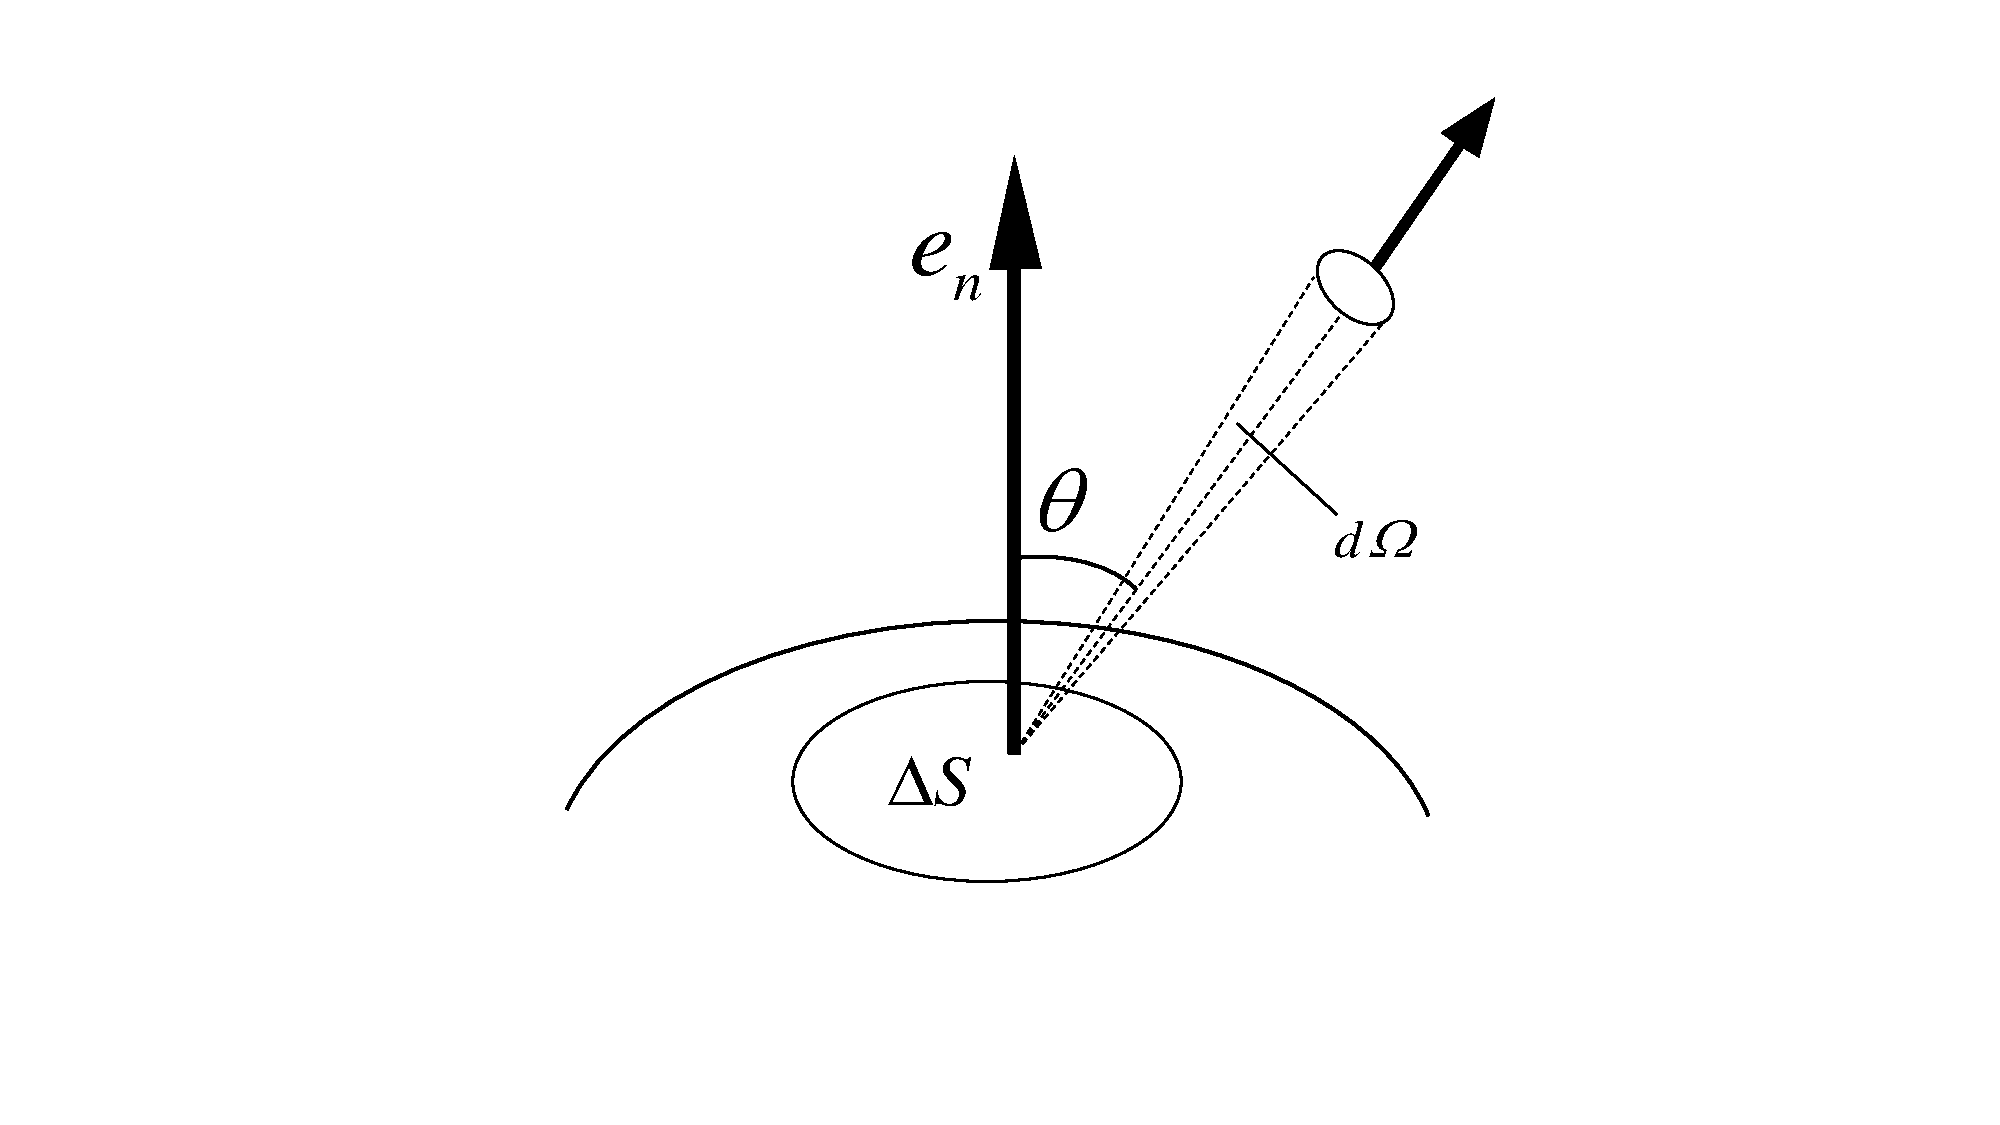
\includegraphics[width=2.5cm]{QM file/figure/1-1}
	\caption{}\label{fig.1-1}
\end{wrapfigure}
\eqindent{4}
\begin{equation*}
	\sigma=5.6704 \times 10^{-8} \si{W\cdot m^{-2} \cdot K^{-4}} 
\end{equation*}\eqnormal

图\ref{fig.1-1}是黑体辐射示意图,将空腔加热至温度$T$,这时腔内电磁场具有稳定的能量分布(各种频率的电磁波),经由小孔 $\Delta S$辐射出的能流可用仪器测出.如以$u$表示腔内电磁场能量密度(单位体积内电磁波能量),$c$表示光速,则单位时间内由$\Delta S$沿$d \Omega$方向辐射出的能量为
\begin{equation*}
	\Delta S\cdot \cos\theta\cdot cu\frac{d\Omega}{4\pi}
\end{equation*}
经$\Delta S$辐射出的总能量为
\begin{equation*}
	\begin{aligned}
		J_{u}\Delta S &=\int_{\theta \leq\frac{\pi}{2}}\Delta S \cos\theta cu \frac{d\Omega}{4\pi} \\
		&=\Delta S cu\frac{1}{4\pi}\int_{0}^{2\pi}d\varphi \int_{0}^{\frac{\pi}{2}}\cos\theta\sin\theta d\theta \\
		&= \frac{1}{4}cu\Delta S \\
	\end{aligned}
\end{equation*}
因此
\eqshort
\begin{equation}\label{eq11.02}
	u=\frac{4}{c}J_{u}=\frac{4\sigma}{c}T^{4}
\end{equation}
热辐射电磁场的能量密度与温度4次方成正比.注意比例系数为普适常数.

实验还可以测量出热辐射能量的频率分布.电磁波的波长$\lambda$与频率$\nu$及角频率$\omega=2\pi\nu$间有如下关系:
\begin{equation}\label{eq11.03}
	c=\lambda\nu=\frac{\lambda \omega}{2\pi}
\end{equation}
如以$\rho(\omega)d\omega$表示单位体积内角频率在$(\omega,\omega+d\omega)$间的电磁波能量,则能量密度$u$按$\omega$分布可以表示成
\begin{equation}\label{eq11.04}
	u=\int_{0}^{u} \rho(\omega)d\omega
\end{equation}\eqnormal
\begin{wrapfigure}[9]{r}{9em}
	\centering
	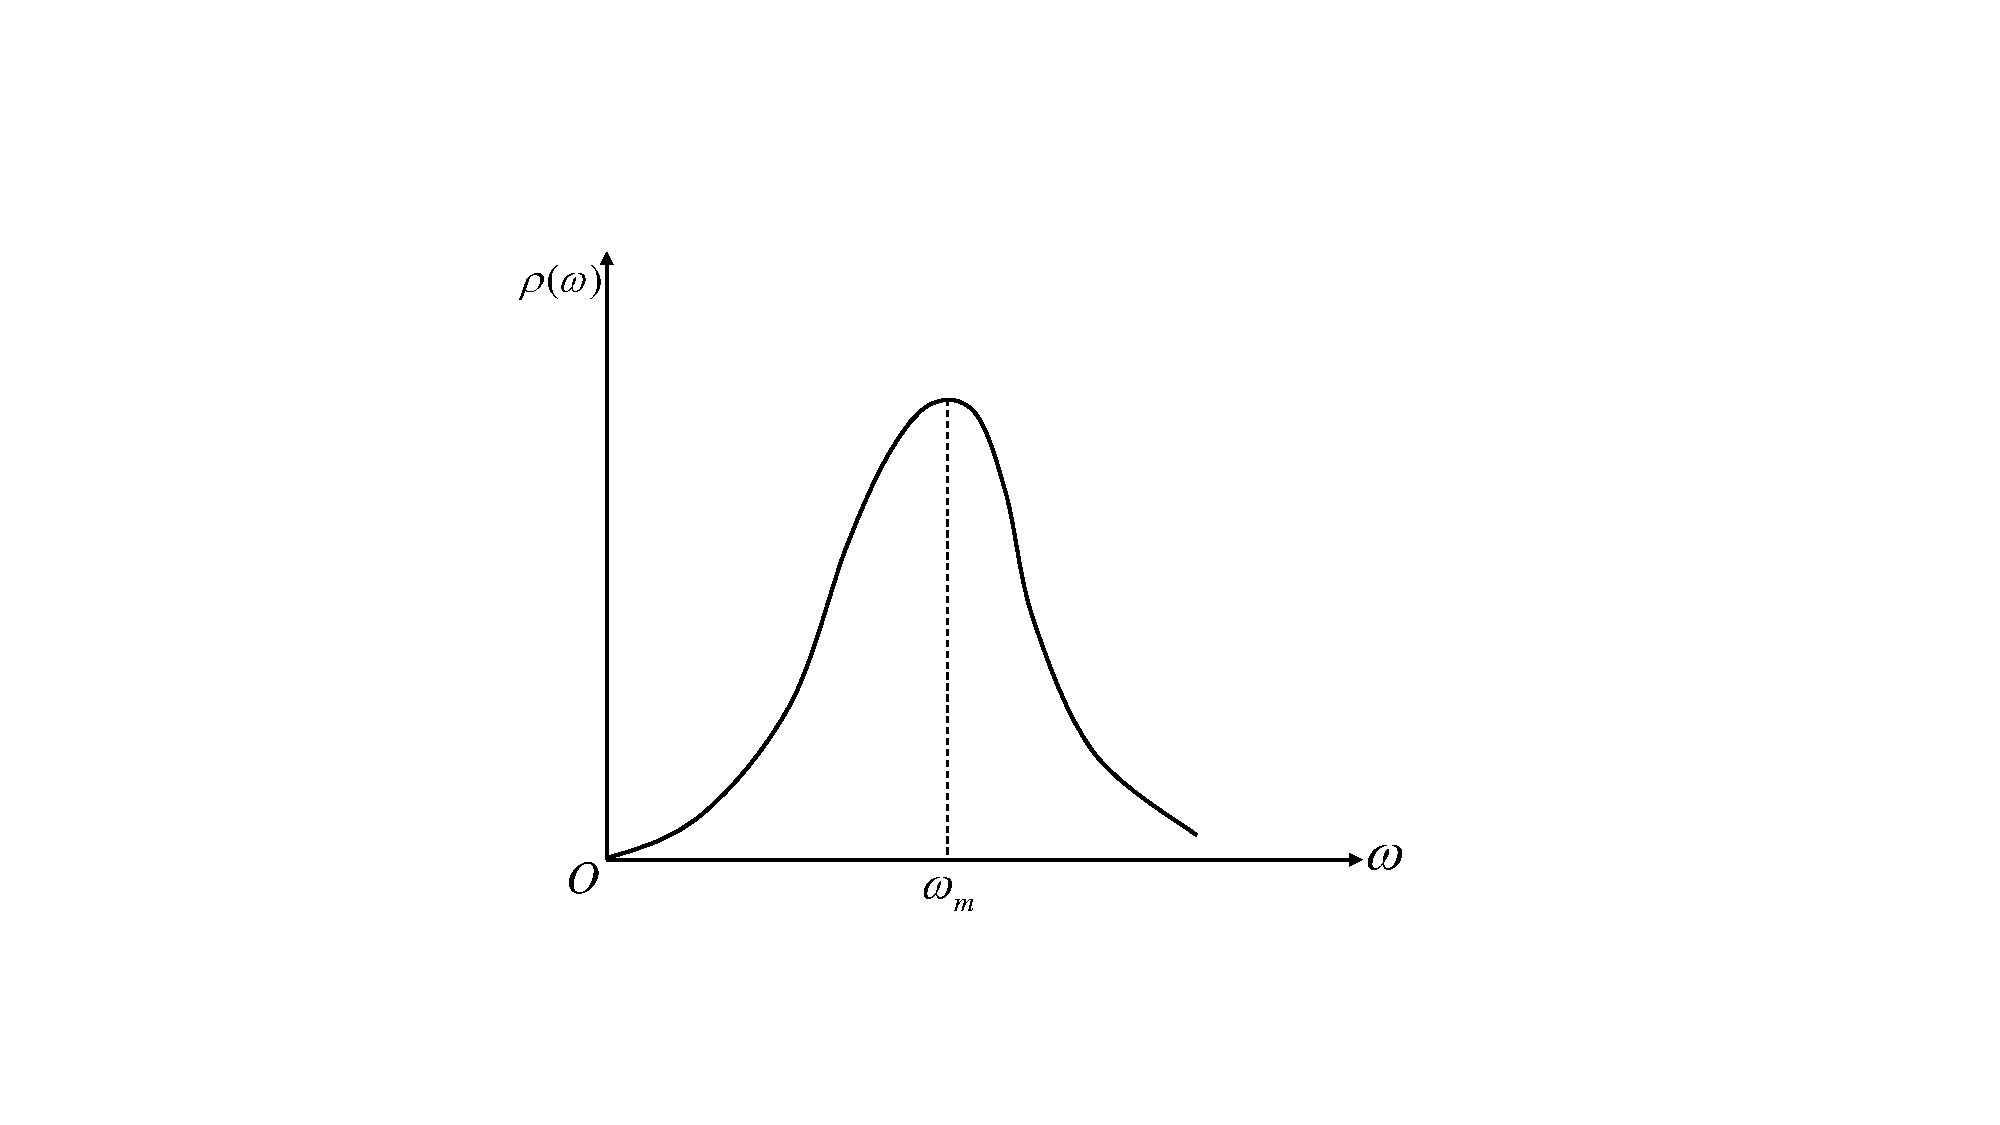
\includegraphics[width=3.5cm]{QM file/figure/1-2}
	\caption{}\label{fig.1-2}
\end{wrapfigure}

实验测得各种温度下$u$的频率分布曲线如图\ref{fig.1-2}所示.在长波部分$(\omega \rightarrow 0)\rho(\omega)\propto \omega^{2}T$;在短波部分$(\omega\rightarrow\infty)\rho(\omega)$随$\omega$之增大而迅速减小.对于每一种温度,$\rho(\omega)$都存在一个极大值,相应的角频率$\omega_{m}$和温度$T$成正比,相应的波长$(\lambda_{m}=\frac{2\pi c}{\omega_{m}})$和温度$T$成反比,
\eqindent{5}
\begin{equation}\label{eq11.05}
	T\lambda_{m}=5.1\times 10^{-3}  \si{m\cdot K}
\end{equation}\eqnormal
这规律称为维恩(W.Wein)位移定律.注意\eqref{eq11.05}式中的实验常数也是普适常量.

黑体辐射定律的发现引起了物理学界的极大关注,吸引力许多著名学者对它进行深入的理论探讨.当时经典物理学(牛顿力学,电磁学,热力学和经典统计物理是其主要内容)已经日臻成熟,权威物理学家大多相信经典物理学能够解释各类物理现象,黑体辐射定律应该也不例外.然而,冷酷的事实确是,企图在经典物理的理论框架内解释黑体辐射定律的努力,都在不同程度上遭到失败,其中最有成效的是瑞利和金斯(Rayleigh-Jeans)的研究.金斯利用波动理论,准确求得单位体积内$(\omega,\omega+d\omega)$范围内电磁振动模式总数,它等于
\eqindent{12}
\begin{equation}\label{eq11.06}
	\frac{\omega^{2}d\omega}{\pi^{2}c^{3}}
\end{equation}
\eqnormal
每一种电磁振动模式相当于一个简谐振子,在温度$T$下应该具有某种能量.按照经典统计物理的“能量均分定理”,温度$T$下简谐振子应该具有平均能量$kT$(k是玻尔兹曼常数).瑞利将“能量均分定理”用于热平衡下的电磁场(即热辐射场),从而得出结论:单位体积内$\omega,\omega+d\omega$范围内电磁振动能量应该是
\begin{equation}\label{eq11.07}
	\rho(\omega)d\omega=\frac{kT\omega^{2}d\omega}{\pi^{2}c^{3}}
\end{equation} 
这称为瑞利-金斯公式.这个公式在长波部分和实验曲线符合得极好,而在短波部分则和实验结果完全不符合.更严重的是,\eqref{eq11.07}式对$\omega$积分,将导致$u\rightarrow\infty$,这个结论显然是错误的.这就是历史上有名的“紫外发散困难”.

经历了许多失败,终于使物理学界认识到,为了解释黑体辐射定律,光靠经典物理学是不行的,必须有一个新的理论.这就是1900年普朗克(M.Planck)提出的量子论.

普朗克量子论的核心是下述“量子假设”:频率为$\nu$的电磁振动和原子、分子等物质发生能量转换时,能量不能连续变化,只能“量子”式地变化,每份“能量子”为
\begin{equation}\label{eq11.08}
	\varepsilon=h\nu=\hbar\omega \quad(\hbar=\frac{h}{2\pi})
\end{equation}
其中$h$是普适常数(后人称之为普朗克常数).在这假设下,普朗克利用热力学和统计物理理论,导出了著名地普朗克公式
\begin{equation}\label{eq11.09}
	\boxed{\rho(\omega)=\frac{\hbar\omega^{3}}{\pi^{2}c^{3}} \bigg/ (e^{\hbar\omega/kT}-1)}
\end{equation}

这个公式在各种温度下,全部频率范围内,均与实验曲线精确符合.历史上,普朗克导出\eqref{eq11.09}式的过程相当复杂.$\S$\ref{sec:09.04}将给出爱因斯坦对此式的简单证明.

普朗克的“量子假设”是和经典物理的整套概念抵触的.按照经典物理学,一切物质的运动变化都是连续进行的,能量变化也是连续的,这正是导致热平衡下“能量均分定理”的前提条件.普朗克舍弃了“能量均分定理”,代之以“量子假设”这在概念上是一次革命性的突破.从\eqref{eq11.09}式的结果看,由于能量的量子化,角频率为$\omega$的每一种电磁振动模式在温度$T$下的平均能量不再取“能量均分定理”给出的$kT$,而是
\begin{equation*}
	 E_{\omega}=\frac{\hbar\omega}{e^{\hbar\omega/kT}-1} 
\end{equation*}
在长波部分,$\hbar\omega\ll kT$,上式给出$\bar{E}_{\omega}\simeq kT$,与能量均分定理的结论一致.在短波部分,$\hbar\omega\gg kT$,上式给出
\begin{equation*}
	 \bar{E}_{\omega}\simeq \hbar\omega e^{\hbar\omega/kT} \ll kT 
\end{equation*}
这意味着高频振动被“冻结”,很难获得能量,因此避免了“紫外发散困难”.当一种电磁振动模式(角频率$\omega$)具有能量$E_{\omega}$时,相应的“能量子”数目为$n_{\omega}=\frac{E_{\omega}}{\hbar\omega}$,\eqref{eq11.09}式相当于“能量子”数的平均值为
\eqshort
\begin{equation}\label{eq11.10}
	\bar{n}_{\omega}=\frac{1}{e^{\hbar\omega/kT}-1}
\end{equation}
当$\hbar\omega\ll kT$,$\bar{n}_{\omega}=\simeq\frac{kT}{\hbar\omega}\gg 1$,电磁振动的能量变化近似于连续变化,量子论的结果和经典物理结果一致,当$\hbar\omega\gtrsim kT$,$\bar{n}_{\omega}<1$,量子论的结果和经典物理结果有本质差别.

\eqref{eq11.09}式代入\eqref{eq11.04}式,可以算出热辐射电磁场能量密度:
\begin{equation}\label{eq11.11}
	u=\frac{\pi^{2}(kT)^{4}}{15(\hbar c)^{3}}
\end{equation}\eqnormal
这结果与斯特藩-玻尔兹曼定律一致.

普朗克的“量子假设”是与整个经典物理格格不入的,使许多习惯于经典物理思维模式的资深物理学家感到难以接受.普朗克本人就曾花了多年时间研究能否不要“量子假设”,而在经典物理的范围内导出\eqref{eq11.09}式,结论是不能.显然,这意味着黑体辐射现象的后面隐藏着一种新的物理规律,这就是今天所谓的量子力学规律.

在这里,我们将用量纲分析方法证明黑体辐射定律绝不可能在经典物理学的框架范围内得到解释.

物理学的发展历史表明,每一种基本物理规律,均伴有相应的普适常数.例如代表万有引力定律的普适常数是引力常数$G$,代表电磁规律和相对论的基本普适常数是光速$c$,代表统计物理规律的基本普适常数是玻尔兹曼常数$k$,等等.如果黑体辐射定律可由经典物理来解释,有关的理论将是电磁学和统计物理,则在辐射场能量密度$u$的构造式中,只能包含$c,k,T$ $L,t,E,K$分别表示长度,时间,能量,温度的量纲,有关各量的量纲如下:
\begin{gather*}
	u——  \si{EL^{-3}},\qquad \qquad c——  \si{Lt^{-1}}  \\
	k——  \si{EK^{-1}},\qquad \qquad kT—— \si{E}  \\
	\sigma——  \si{Et^{-1}L^{-2}K^{-4}}
\end{gather*}
从量纲关系看,$u$显然不能由$c,k,T$构成,$\sigma$(普适常数)不可能由$c,k$构成.根据\eqref{eq11.02}式,可以判断$u\propto(kT)^{4}$,而从$u,c$与长度的量纲关系来看,可以设想$u\propto c^{-3}$,因此,$u\propto(kT)^{4}c^{-3}$.而$uc^{3}(kT)^{-4}$的量纲为$\si{(Et)^{-3}}$.如果设想黑体辐射现象涉及一种新的(未知的)基本物理规律,相应的基本普适常量(记为$\hbar$)量纲为$\si{Et}$,则$u$的构造式可以设想为
\eqshort
\begin{equation}\label{eq11.12}
	u=A(kT)^{4}(\hbar c)^{-3}
\end{equation}
其中$A$为无量纲纯数,结合\eqref{eq11.02}式,可得斯特藩-玻尔兹曼常数的构造式为
\begin{equation}\label{eq11.13}
	\sigma=\frac{A}{4}k^{4}\hbar^{-3}c^{-2}
\end{equation}\eqnormal
读者当然已经想到,这里提到的代表新规律的基本普适常数$\hbar$正好就是普朗克常数.事实上,如略去\eqref{eq11.12}、\eqref{eq11.13}式中不太重要的纯数$A$,利用$c,k,\sigma$的实验值,由\eqref{eq11.13}式即可估算出$\hbar \sim1.2\times 10^{-34} \si{J\cdot s}$,这正是普朗克常数$\frac{h}{2\pi}$的量级.如按精确计算得到的\eqref{eq11.11}式,[相当于\eqref{eq11.12}、\eqref{eq11.13}式中取$A=\frac{\pi^{2}}{15}$]则如上所述可以算出
\setlength{\mathindent}{4em}
\begin{equation*}
	\hbar=1.0546\times 10^{-34} \si{J\cdot s},\quad h=2\pi\hbar=6.6262\times 10^{-34} \si{J\cdot s}
\end{equation*}
\setlength{\mathindent}{9em}
这数值与普朗克常数的精密测量值非常接近.

\example 试用普朗克公式\eqref{eq11.09}求$\rho(\omega)$极大值对应的角频率$\omega_{m}$与温度$T$的数值关系,并估算热辐射场的光子数密度.

\solution $\rho(\omega)$取极大值时,满足极值条件$\frac{\partial \rho}{\partial \omega}=0$.令$x=\frac{\hbar\omega}{kT}$,极值条件亦即
\eqshort
\begin{equation*}
	\frac{d}{dx}\frac{x^{3}}{e^{x}-1}=0
\end{equation*}
由此得出$x$满足的方程为
\begin{equation*}
	\frac{x}{3}=1-e^{-x}
\end{equation*}
用数值解法可解出$x=\num{2.8214}$,因此
\begin{equation}\label{eq11.14}
	\frac{\hbar\omega_{m}}{kT}=\num{2.8214}
\end{equation}\eqnormal
这正是维恩位移定律.读者不难验证\eqref{eq11.14}式与\eqref{eq11.05}式是一致的.

由于辐射场的能量集中分布在$\omega\sim\omega_{m}$附近,所以光子数密度(单位体积内光子数)可估计成
\begin{equation}\label{eq11.15}
	n\sim\frac{u}{\hbar\omega_{m}}\sim\frac{\pi^{2}}{15\times2.82}\bigl(\frac{kT}{\hbar c}\bigr)^{3}\sim 0.23\bigl(\frac{kT}{\hbar c}\bigr)^{3}
\end{equation}
精确结果是
\begin{equation}\label{eq11.16}
	n=\int_{0}^{\infty}\frac{\rho(\omega)}{\hbar\omega}d\omega=0.2436\bigl(\frac{kT}{\hbar c}\bigr)^{3}
\end{equation}

从量纲关系看,$n$的构造式中只能包含$kT,c,\hbar$,他们的量纲是
\begin{equation*}
	n——\si{L^{-3}},\quad kT—— \si{E},\quad \hbar c—— \si{EL} 
\end{equation*}
所以唯一可能的量纲构造关系是$n\sim\bigl( \frac{kT}{\hbar c} \bigr)^{3}$







